% !TEX root = ../discretemath.tex

\section{Функция Мёбиуса на частично упорядоченных множествах}

\subsection{Частично упорядоченные множества}

\begin{Definition}{Частично упорядоченное множество (ЧУМ)}{}
	Множество $P$ с отношением строгого порядка~$<$ называется
	\emph{частично упорядоченным множеством} (ЧУМ), если выполнены:
	\begin{enumerate}
		\item \textbf{Иррефлексивность:} $x \not< x$ для всех $x \in P$.
		\item \textbf{Антисимметричность:} $x < y$ и $y < x$ одновременно невозможны.
		\item \textbf{Транзитивность:} если $x < y$ и $y < z$, то $x < z$.
	\end{enumerate}
	Пишем $x \leq y$, если $x < y$ или $x = y$.
	
	Для $x,y \in P$, $x \le y$, отрезком называется множество
	\[
	[x,y] = \{z \in P \mid x \le z \le y\}.
	\]
	Будем рассматривать только такие ЧУМы, для которых каждый отрезок $[x,y]$ конечен.
\end{Definition}

\subsection{Функция Мёбиуса}

\begin{Definition}{Функция Мёбиуса ЧУМа}{}
	Пусть $P$~--- ЧУМ. \emph{Функция Мёбиуса} $\mu \colon P \times P \to \mathbb{Z}$
	определяется рекурсивно:
	\[
	\mu(x,\, y)
	\;=\;
	\begin{cases}
		1,
		& \text{если } x = y,\\[6pt]
		-\displaystyle\sum_{x \leq z < y}\mu(x,z),
		& \text{если } x < y,\\[6pt]
		0,
		& \text{иначе.}
	\end{cases}
	\]
\end{Definition}

\begin{Corollary}{}{}
	Для функции Мёбиуса $\mu$ следующие условия эквивалентны:
	\[
	\mu(x,x)=1 \quad \text{для всех } x \in P,
	\]
	и при $x<y$
	\[
	\sum_{x \leq z \leq y} \mu(x,z)=0.
	\]
\end{Corollary}

Это непосредственно следует из определения: $\mu(x,y) = -\!\sum_{x \leq z < y}\mu(x,z)$,
поэтому $\sum_{x \leq z \leq y}\mu(x,z) = \mu(x,y) + \sum_{x \leq z < y}\mu(x,z) = 0$.

\begin{Remark}{}{}
	Функция Мёбиуса существует и единственна.
	
	Действительно, при $x=y$ её значение равно $1$, при $x \nleq y$ равно $0$,
	а при $x<y$ значение $\mu(x,y)$ однозначно выражается через значения
	$\mu(x,z)$ для $z<y$. Поскольку ЧУМ локально конечен, все возникающие суммы конечны, и рекурсия корректно задаёт функцию на всех парах $(x,y)$.
\end{Remark}
\subsection{Примеры}

\begin{Example}{Пятиэлементный ЧУМ}{}
	Рассмотрим множество $\{0, a, b, c, d\}$ с отношениями
	$0 < a < d$ и $0 < b < c < d$, где $a$ и $c$ несравнимы
	(так называемая «пятиугольная» диаграмма Хассе).
	
	\begin{center}
		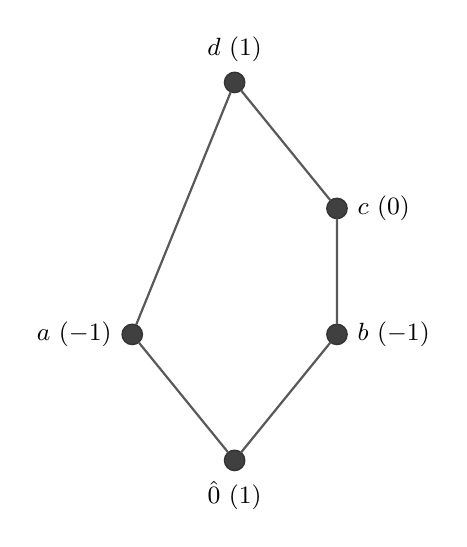
\begin{tikzpicture}[
			scale=1,
			nd/.style={
				circle, draw=black!80, fill=black!75,
				inner sep=2.6pt, line width=0.5pt
			},
			lbl/.style={font=\small},
			edge/.style={thick, draw=black!65, line cap=round}
			]
			
			\node[nd, label={[lbl]below:$\hat{0}\ (1)$}]   (bot) at ( 0.0, 0.0) {};
			\node[nd, label={[lbl]left:$a\ ({-1})$}]        (a)   at (-1.3, 1.6) {};
			\node[nd, label={[lbl]right:$b\ ({-1})$}]       (b)   at ( 1.3, 1.6) {};
			\node[nd, label={[lbl]right:$c\ (0)$}]          (c)   at ( 1.3, 3.2) {};
			\node[nd, label={[lbl]above:$d\ (1)$}]          (top) at ( 0.0, 4.8) {};
			
			\draw[edge] (bot)--(a)--(top);
			\draw[edge] (bot)--(b)--(c)--(top);
			
		\end{tikzpicture}
	\end{center}
	
	В скобках у каждого элемента указано значение $\mu(0,\cdot)$.
	Проверим по определению:
	\begin{align*}
		\mu(0,0) &= 1,\\
		\mu(0,a) &= -\mu(0,0) = -1,\\
		\mu(0,b) &= -\mu(0,0) = -1,\\
		\mu(0,c) &= -\bigl(\mu(0,0)+\mu(0,b)\bigr) = -(1 - 1) = 0,\\
		\mu(0,d) &= -\bigl(\mu(0,0)+\mu(0,a)+\mu(0,b)+\mu(0,c)\bigr)
		= -(1 - 1 - 1 + 0) = 1.
	\end{align*}
\end{Example}

\subsubsection*{Функция Мёбиуса булевой решётки}

\begin{Example}{Булева решётка $2^{\{1,\ldots,n\}}$}{}
	Пусть $P = 2^{\{1,\ldots,n\}}$~--- множество всех подмножеств
	$\{1,\ldots,n\}$, упорядоченных по включению: $A \leq B \Leftrightarrow A \subseteq B$.
\end{Example}

\begin{Theorem}{Функция Мёбиуса булевой решётки}{}
	В булевой решётке $2^{\{1,\ldots,n\}}$:
	\[
	\mu(A,B)
	\;=\;
	\begin{cases}
		(-1)^{|B|-|A|}, & \text{если } A \subseteq B,\\
		0,              & \text{иначе.}
	\end{cases}
	\]
\end{Theorem}

\begin{proof}
	Доказательство ведётся индукцией по $|B \setminus A|$.
	
	\textbf{База.} При $A = B$: $\mu(A,A) = 1 = (-1)^0$.\;\checkmark
	
	\textbf{Переход.} Пусть $A \subsetneq B$. По определению:
	\[
	\mu(A,B)
	= -\sum_{A \subseteq C \subsetneq B}\mu(A,C)
	\stackrel{\text{(ИП)}}{=}
	-\sum_{A \subseteq C \subsetneq B}(-1)^{|C|-|A|}.
	\]
	Обозначим $n = |B|-|A|$. Число множеств $C$ с $A\subseteq C\subsetneq B$
	и $|C|-|A|=k$ равно $\binom{n}{k}$, поэтому:
	\[
	\mu(A,B)
	= -\sum_{k=0}^{n-1}(-1)^k\binom{n}{k}.
	\]
	Из бинома Ньютона при $n \geq 1$:
	\[
	\sum_{k=0}^{n}(-1)^k\binom{n}{k}
	= (1-1)^n = 0
	\;\Longrightarrow\;
	\sum_{k=0}^{n-1}(-1)^k\binom{n}{k}
	= -(-1)^n.
	\]
	Следовательно:
	\[
	\mu(A,B)
	= -\bigl(-(-1)^n\bigr)
	= (-1)^n
	= (-1)^{|B|-|A|}.\;\checkmark
	\]
\end{proof}

\subsection{Лемма о симметричной сумме}

Для доказательства леммы нам потребуется понятие интервала.

\begin{Definition}{Интервал в ЧУМ}{}
	Для $a \leq b$ в $P$ определяется \emph{интервал}
	\[
	(a,b) \;=\; \bigl\{c \in P \;:\; a < c < b\bigr\}.
	\]
\end{Definition}

\begin{Lemma}{}{}
	Для любых $x < y$ в ЧУМ $P$:
	\[
	\sum_{x \leq z \leq y} \mu(z,\, y) = 0.
	\]
\end{Lemma}

\begin{proof}
	Доказательство ведётся индукцией по $|[x,y]|$.
	
	\textbf{База.} $|[x,y]| = 2$, то есть $x < y$ и промежуточных элементов нет.
	Единственный $z < y$ с $z \geq x$ --- это сам $x$:
	\[
	\sum_{x \leq z \leq y}\mu(z,y)
	= \mu(x,y) + \mu(y,y)
	= -\mu(x,x) + 1
	= -1 + 1 = 0.\;\checkmark
	\]
	
	\textbf{Переход.} Пусть $|[x,y]| > 2$. Выделим слагаемое при $z=y$:
	\[
	\sum_{x \leq z \leq y}\mu(z,y)
	= \sum_{x \leq z < y}\mu(z,y) + 1.
	\]
	Для каждого $z < y$ по определению функции Мёбиуса:
	\[
	\mu(z,y) = -\sum_{z \leq u < y}\mu(z,u).
	\]
	Подставляем и меняем порядок суммирования по парам $(z,u)$ с $x \leq z \leq u < y$:
	\begin{align*}
		\sum_{x \leq z < y}\mu(z,y)
		&= -\sum_{x \leq z < y}\;\sum_{z \leq u < y}\mu(z,u)
		= -\sum_{x \leq u < y}\;\sum_{x \leq z \leq u}\mu(z,u).
	\end{align*}
	Оцениваем внутреннюю сумму:
	\begin{itemize}
		\item при $u = x$: $\displaystyle\sum_{x \leq z \leq x}\mu(z,x) = \mu(x,x) = 1$;
		\item при $x < u < y$: интервал $[x,u]$ строго меньше $[x,y]$,
		поэтому по ИП $\displaystyle\sum_{x \leq z \leq u}\mu(z,u) = 0$.
	\end{itemize}
	Следовательно:
	\[
	\sum_{x \leq z \leq y}\mu(z,y)
	= -\bigl(1 + 0 + \cdots + 0\bigr) + 1
	= -1 + 1 = 0.\;\checkmark
	\]
\end{proof}

\subsection{Двойственный ЧУМ}

\begin{Definition}{Двойственный ЧУМ}{}
	Если $P$~--- ЧУМ, то \emph{двойственный ЧУМ} $P^*$~--- то же множество с обратным порядком:
	\[
	x \leq^* y \;\Longleftrightarrow\; x \geq y \quad\text{в } P.
	\]
	Функцию Мёбиуса ЧУМа $P^*$ обозначаем $\mu^*$.
\end{Definition}

\begin{Theorem}{Функция Мёбиуса двойственного ЧУМа}{}
	Пусть $P$~--- ЧУМ, $P^*$~--- двойственный к нему. Тогда
	\[
	\mu_P(a,\, b) \;=\; \mu^*(b,\, a).
	\]
\end{Theorem}

\begin{proof}
	Покажем, что функция $f(a,b) := \mu^*(b,a)$ удовлетворяет тем же начальным условиям
	и рекуррентному соотношению, что и $\mu_P(a,b)$.
	\begin{itemize}
		\item $f(a,a) = \mu^*(a,a) = 1$.\;\checkmark
		\item Для $a < b$ в $P$ (т.е. $b <^* a$ в $P^*$) по лемме о симметричной сумме,
		применённой к $P^*$:
		\[
		\sum_{x \leq^* z \leq^* y}\mu^*(z,\,y) = 0
		\;\Longrightarrow\;
		\sum_{a \leq z \leq b}f(a,z)
		= \sum_{a \leq z \leq b}\mu^*(z,\,a) = 0.
		\]
	\end{itemize}
	Из единственности функции Мёбиуса заключаем $\mu_P(a,b) = \mu^*(b,a)$.
\end{proof}

\subsection{Прямое произведение ЧУМ}

\begin{Definition}{Прямое произведение ЧУМ}{}
	Пусть $A$ и $B$~--- два ЧУМа. \emph{Прямое произведение} $A \times B$~---
	ЧУМ на парах $(a,b) \in A\times B$ с покоординатным порядком:
	\[
	(a,b) \leq (a',b')
	\;\Longleftrightarrow\;
	a \leq_A a' \;\text{ и }\; b \leq_B b'.
	\]
\end{Definition}

\begin{Theorem}{Мультипликативность функции Мёбиуса}{}
	\[
	\mu_{A\times B}\!\bigl((a,b),\,(a',b')\bigr)
	\;=\;
	\mu_A(a,a')\cdot\mu_B(b,b').
	\]
\end{Theorem}

\begin{proof}
	Доказательство ведётся индукцией по размеру интервала $[(a,b),(a',b')]$ в $A\times B$.
	
	\textbf{База.} $a = a'$ или $b = b'$.
	
	Если $a = a'$, то $[(a,b),(a,b')] \cong [b,b']$ в $B$, откуда
	\[
	\mu_{A\times B}\!\bigl((a,b),(a,b')\bigr)
	= \mu_B(b,b')
	= \underbrace{\mu_A(a,a)}_{=\,1}\cdot\mu_B(b,b').
	\]
	Случай $b = b'$ аналогичен.\;\checkmark
	
	\textbf{Переход.} $a < a'$ и $b < b'$.
	
	Из следствия об обнулении суммы, применённого в $A\times B$:
	\[
	\sum_{\substack{a \leq s \leq a' \\ b \leq t \leq b'}}
	\mu_{A\times B}\!\bigl((a,b),(s,t)\bigr) = 0.
	\]
	По индукционному предположению (для всех $(s,t)\neq(a',b')$):
	$\mu_{A\times B}((a,b),(s,t)) = \mu_A(a,s)\cdot\mu_B(b,t)$.
	Отсюда:
	\begin{align*}
		\mu_{A\times B}\!\bigl((a,b),(a',b')\bigr)
		&= -\!\sum_{\substack{a\leq s\leq a',\;b\leq t\leq b'\\(s,t)\neq(a',b')}}
		\mu_A(a,s)\cdot\mu_B(b,t)\\
		&= \mu_A(a,a')\cdot\mu_B(b,b')
		\;-\!\sum_{\substack{a\leq s\leq a'\\b\leq t\leq b'}}
		\mu_A(a,s)\cdot\mu_B(b,t)\\
		&= \mu_A(a,a')\cdot\mu_B(b,b')
		\;-\;\Bigl(\sum_{a\leq s\leq a'}\mu_A(a,s)\Bigr)
		\!\cdot\!\Bigl(\sum_{b\leq t\leq b'}\mu_B(b,t)\Bigr)\\
		&= \mu_A(a,a')\cdot\mu_B(b,b') - 0\cdot 0
		= \mu_A(a,a')\cdot\mu_B(b,b').\;\checkmark
	\end{align*}
\end{proof}

\subsection{Формула обращения Мёбиуса}

\begin{Definition}{Укороченное обозначение $\hat{\mu}$}{}
	Пусть $P$~--- ЧУМ с минимальным элементом $\hat{0}$. Введём сокращение:
	\[
	\hat{\mu}(x) \;:=\; \mu(\hat{0},\, x).
	\]
\end{Definition}

\begin{Theorem}{Формула обращения Мёбиуса}{}
	Пусть $P$~--- ЧУМ с минимальным элементом $\hat{0}$, и пусть $f, g \colon P \to \mathbb{R}$.
	Тогда следующие два условия равносильны:
	\begin{enumerate}
		\item $\forall x \in P\colon\quad f(x) = \displaystyle\sum_{z \leq x} g(z)$,
		\item $\forall x \in P\colon\quad g(x) = \displaystyle\sum_{z \leq x} \mu(z,\, x)\, f(z)$.
	\end{enumerate}
	
	Здесь, поскольку $\hat{0}$~--- минимальный элемент, условие $z\le x$ равносильно
	условию $\hat{0}\le z\le x$, так что суммирование фактически ведётся по отрезку
	$[\hat{0},x]$.
\end{Theorem}

\begin{proof}
	\textbf{(1) $\Rightarrow$ (2).}
	Подставим $f(z) = \sum_{y \leq z} g(y)$ в правую часть условия~(2):
	\begin{align*}
		\sum_{z \leq x} \mu(z,x)\,f(z)
		&= \sum_{z \leq x} \mu(z,x) \sum_{y \leq z} g(y)
		= \sum_{\substack{y,z\\y \leq z \leq x}} \mu(z,x)\,g(y)
		= \sum_{y \leq x} \Bigl(\sum_{y \leq z \leq x} \mu(z,x)\Bigr) g(y).
	\end{align*}
	По лемме о симметричной сумме:
	\[
	\sum_{y \leq z \leq x} \mu(z,x)
	= \begin{cases} 0, & y < x, \\ 1, & y = x. \end{cases}
	\]
	Следовательно, вся сумма равна $g(x)$.\;\checkmark
	
	\medskip
	\textbf{(2) $\Rightarrow$ (1).}
	Подставим $g(z) = \sum_{y \leq z} \mu(y,z)\,f(y)$ в правую часть условия~(1):
	\begin{align*}
		\sum_{z \leq x} g(z)
		&= \sum_{z \leq x} \sum_{y \leq z} \mu(y,z)\,f(y)
		= \sum_{y \leq x} \Bigl(\sum_{y \leq z \leq x} \mu(y,z)\Bigr) f(y).
	\end{align*}
	По следствию об обнулении суммы:
	\[
	\sum_{y \leq z \leq x} \mu(y,z)
	= \begin{cases} 0, & y < x, \\ 1, & y = x. \end{cases}
	\]
	Следовательно, вся сумма равна $f(x)$.\;\checkmark
\end{proof}

\subsection{Классическая функция Мёбиуса}

\subsubsection*{ЧУМ натуральных чисел по делимости}

Рассмотрим ЧУМ $(\mathbb{N},\,|\,)$: множество натуральных чисел с порядком
$a \leq b \Leftrightarrow a \mid b$. Ниже изображена часть диаграммы Хассе.

\begin{center}
	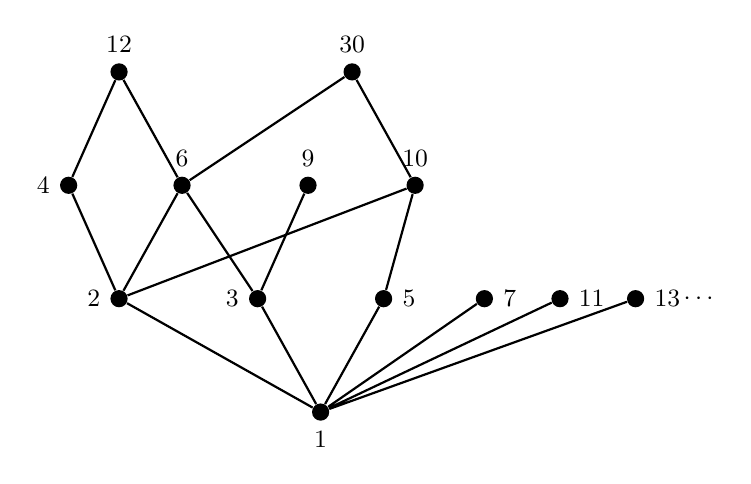
\begin{tikzpicture}[
		nd/.style   = {circle, fill=black, inner sep=2.2pt},
		lbl/.style  = {font=\small},
		every label/.style = {font=\small},
		scale = 0.8
		]
		\node[nd, label={[lbl]below:$1$}]    (n1)  at ( 0.0, 0.0) {};
		
		\node[nd, label={[lbl]left:$2$}]     (n2)  at (-3.2, 1.8) {};
		\node[nd, label={[lbl]left:$3$}]     (n3)  at (-1.0, 1.8) {};
		\node[nd, label={[lbl]right:$5$}]    (n5)  at ( 1.0, 1.8) {};
		\node[nd, label={[lbl]right:$7$}]    (n7)  at ( 2.6, 1.8) {};
		\node[nd, label={[lbl]right:$11$}]   (n11) at ( 3.8, 1.8) {};
		\node[nd, label={[lbl]right:$13$}]   (n13) at ( 5.0, 1.8) {};
		\node[lbl] at (6.0, 1.8) {$\cdots$};
		
		\node[nd, label={[lbl]left:$4$}]     (n4)  at (-4.0, 3.6) {};
		\node[nd, label={[lbl]above:$6$}]    (n6)  at (-2.2, 3.6) {};
		\node[nd, label={[lbl]above:$9$}]    (n9)  at (-0.2, 3.6) {};
		\node[nd, label={[lbl]above:$10$}]   (n10) at ( 1.5, 3.6) {};
		
		\node[nd, label={[lbl]above:$12$}]   (n12) at (-3.2, 5.4) {};
		\node[nd, label={[lbl]above:$30$}]   (n30) at ( 0.5, 5.4) {};
		
		\draw[thick] (n1)--(n2)  (n1)--(n3)  (n1)--(n5)
		(n1)--(n7)  (n1)--(n11) (n1)--(n13);
		
		\draw[thick] (n2)--(n4)  (n2)--(n6)  (n2)--(n10);
		\draw[thick] (n3)--(n6)  (n3)--(n9);
		\draw[thick] (n5)--(n10);
		
		\draw[thick] (n4)--(n12) (n6)--(n12);
		\draw[thick] (n6)--(n30) (n10)--(n30);
	\end{tikzpicture}
\end{center}

\begin{Definition}{Классическая функция Мёбиуса}{}
	\emph{Классическая функция Мёбиуса} $\mu \colon \mathbb{N} \to \{-1,0,1\}$:
	\[
	\mu(n) \;=\;
	\begin{cases}
		0,        & \text{если } p^2 \mid n
		\text{ для некоторого простого } p,\\[5pt]
		(-1)^{k}, & \text{если } n = p_1 p_2 \cdots p_k
		\text{ --- произведение $k$ различных простых.}
	\end{cases}
	\]
	В частности, $\mu(1) = 1$.
\end{Definition}

\begin{Theorem}{Связь с функцией Мёбиуса ЧУМа}{}
	Для любых $a \mid b$ в $(\mathbb{N},\,|\,)$:
	\[
	\mu_{\mathbb{N}}(a,\, b) \;=\; \mu\!\left(\tfrac{b}{a}\right).
	\]
\end{Theorem}

Это следует из изоморфизма интервалов: $[a,\, b] \;\cong\; \Bigl[1,\, \tfrac{b}{a}\Bigr],$ откуда $\mu_{\mathbb{N}}(a,b) = \mu_{\mathbb{N}}\!\left(1,\,\dfrac{b}{a}\right) =: \mu\!\left(\dfrac{b}{a}\right)$.

\subsubsection*{Вычисление $\mu(1, n)$}

Пусть $n = p_1^{\alpha_1} \cdots p_k^{\alpha_k}$. Из мультипликативности функции Мёбиуса и изоморфизма
\[
\bigl[1,\; p_1^{\alpha_1}\cdots p_k^{\alpha_k}\bigr]
\;\cong\;
\bigl[1,\, p_1^{\alpha_1}\bigr]
\times \cdots \times
\bigl[1,\, p_k^{\alpha_k}\bigr]
\]
получаем
$\mu\bigl(1,\, n\bigr)
\;=\;
\mu\!\bigl(1,\, p_1^{\alpha_1}\bigr)
\cdots
\mu\!\bigl(1,\, p_k^{\alpha_k}\bigr).$


Каждый множитель вычисляется из цепочки $1 < p_i < p_i^2 < p_i^3 < \cdots$\,:

\begin{center}
	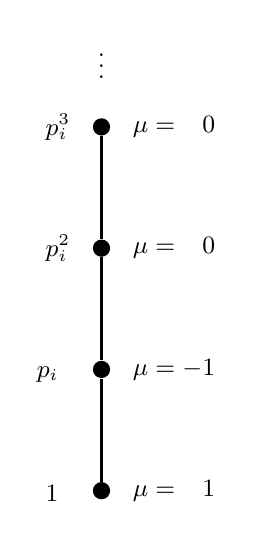
\begin{tikzpicture}[
		nd/.style  = {circle, fill=black, inner sep=2.2pt},
		lbl/.style = {font=\small},
		scale=1.1
		]
		\node[nd] (v0) at (0, 0.0) {};
		\node[nd] (v1) at (0, 1.4) {};
		\node[nd] (v2) at (0, 2.8) {};
		\node[nd] (v3) at (0, 4.2) {};
		
		\draw[thick] (v0)--(v1)--(v2)--(v3);
		\node[font=\small] at (0, 5.0) {$\vdots$};
		
		% Labels left: element
		\node[lbl, anchor=east] at (-0.25, 0.0) {$1\phantom{{}^{3}}$};
		\node[lbl, anchor=east] at (-0.25, 1.4) {$p_i\phantom{{}^{3}}$};
		\node[lbl, anchor=east] at (-0.25, 2.8) {$p_i^2$};
		\node[lbl, anchor=east] at (-0.25, 4.2) {$p_i^3$};
		
		% Labels right: mu value
		\node[lbl, anchor=west] at (0.25, 0.0) {$\mu = \phantom{-}1$};
		\node[lbl, anchor=west] at (0.25, 1.4) {$\mu = -1$};
		\node[lbl, anchor=west] at (0.25, 2.8) {$\mu = \phantom{-}0$};
		\node[lbl, anchor=west] at (0.25, 4.2) {$\mu = \phantom{-}0$};
	\end{tikzpicture}
\end{center}

\begin{itemize}
	\item $\mu(1, p_i) = -\mu(1,1) = -1$.
	\item $\mu(1, p_i^2) = -\mu(1,1) - \mu(1,p_i) = -1+1 = 0$.
	\item По индукции: $\mu(1, p_i^{\alpha}) = 0$ для всех $\alpha \geq 2$.
\end{itemize}

\begin{Corollary}{}{}
	\[
	\mu(1,\, n) \;=\;
	\begin{cases}
		0,        & \text{если } \alpha_i > 1 \text{ хотя бы для одного } i,\\
		(-1)^{k}, & \text{если } \alpha_1 = \cdots = \alpha_k = 1.
	\end{cases}
	\]
	Это в точности классическая функция Мёбиуса $\mu(n)$.
\end{Corollary}

\subsection{Дзета-функция Римана и функция Мёбиуса}

\begin{Definition}{Дзета-функция Римана}{}
	\[
	\zeta(s) \;=\; \sum_{n=1}^{+\infty} \frac{1}{n^s}
	\;=\; \frac{1}{1^s} + \frac{1}{2^s} + \frac{1}{3^s} + \cdots
	\]
\end{Definition}

\begin{Theorem}{}{}
	\[
	\sum_{n=1}^{+\infty} \frac{\mu(n)}{n^s} \;=\; \frac{1}{\zeta(s)}.
	\]
\end{Theorem}

\begin{proof}
	Перемножим ряды $\sum_{n \geq 1}\frac{\mu(n)}{n^s}$ и $\zeta(s) = \sum_{d \geq 1}\frac{1}{d^s}$ и сгруппируем по произведению $m = nd$:
	\[
	\Bigl(\sum_{n=1}^{+\infty} \frac{\mu(n)}{n^s}\Bigr)
	\Bigl(\sum_{d=1}^{+\infty} \frac{1}{d^s}\Bigr)
	\;=\;
	\sum_{m=1}^{+\infty} \frac{1}{m^s}
	\underbrace{\sum_{n \mid m} \mu(n)}_{\displaystyle =\, [m = 1]}.
	\]
	Здесь использован стандартный факт: $\sum_{n \mid m}\mu(n) = 0$ при $m > 1$ и $= 1$ при $m = 1$
	(следствие формулы обращения, применённой к $f \equiv 1$ и $g = [{\cdot} = 1]$). Значит,
	произведение равно $\frac{1}{1^s} = 1$, откуда
	\[
	\sum_{n=1}^{+\infty} \frac{\mu(n)}{n^s}
	\;=\; \frac{1}{\zeta(s)}.\;\checkmark
	\]
\end{proof}

\begin{Theorem}{}{}
	\[
	\sum_{n=1}^{+\infty} \frac{\mu(n)}{n^s} \;=\; \frac{1}{\zeta(s)}.
	\]
\end{Theorem}

\begin{proof}
	Перемножим ряды
	\[
	\sum_{n \geq 1}\frac{\mu(n)}{n^s}
	\qquad \text{и} \qquad
	\zeta(s)=\sum_{d \geq 1}\frac{1}{d^s}
	\]
	и сгруппируем члены по произведению $m=nd$:
	\[
	\Bigl(\sum_{n=1}^{+\infty} \frac{\mu(n)}{n^s}\Bigr)
	\Bigl(\sum_{d=1}^{+\infty} \frac{1}{d^s}\Bigr)
	=
	\sum_{m=1}^{+\infty}\frac{1}{m^s}\sum_{n\mid m}\mu(n).
	\]
	
	Рассмотрим ЧУМ $(\mathbb{N},\mid)$, где порядок задаётся делимостью.
	Тогда условие $n\mid m$ эквивалентно тому, что
	\[
	1 \leq n \leq m
	\qquad \text{в смысле порядка делимости,}
	\]
	то есть $n \in [1,m]$. Поэтому
	\[
	\sum_{n\mid m}\mu(n)=\sum_{1\le n\le m}\mu(1,n).
	\]
	По эквивалентной форме определения функции Мёбиуса эта сумма равна
	\[
	\sum_{1\le n\le m}\mu(1,n)=
	\begin{cases}
		1, & m=1,\\
		0, & m>1.
	\end{cases}
	\]
	Следовательно,
	\[
	\Bigl(\sum_{n=1}^{+\infty} \frac{\mu(n)}{n^s}\Bigr)
	\zeta(s)
	=
	\sum_{m=1}^{+\infty}\frac{1}{m^s}[m=1]
	=1.
	\]
	Отсюда
	\[
	\sum_{n=1}^{+\infty} \frac{\mu(n)}{n^s}
	\;=\;
	\frac{1}{\zeta(s)}.\qedhere
	\]
\end{proof}

\subsection{Арифметические функции}

\begin{Definition}{ Арифметическая (мультипликативная) функция}{}
	Функция $f \colon \mathbb{N} \to \mathbb{Z}$ называется
	\emph{мультипликативной} (арифметической), если для любых
	$m_1, m_2 \in \mathbb{N}$ с $\gcd(m_1, m_2) = 1$:
	\[
	f(m_1 m_2) = f(m_1)\cdot f(m_2).
	\]
\end{Definition}

\begin{Example}{Примеры арифметических функций}{}
	\begin{enumerate}
		\item $f(n) = n^d$ для фиксированного $d \geq 0$ (в частности, $f \equiv 1$ при $d=0$
		и функция тождественного отображения $\mathrm{id}(n) = n$ при $d=1$).
		\item $f(n) = 1$ --- тождественная единица.
		\item $\mu(n)$ --- классическая функция Мёбиуса.
		\item $d(n) = \#\{\text{делители }n\}$ --- количество делителей.
		\item $\varphi(n)$ --- функция Эйлера.
		\item $\sigma(n) = \sum_{d \mid n} d$ --- сумма делителей.
	\end{enumerate}
\end{Example}

\subsection{Свёртка Дирихле}

\begin{Definition}{Свёртка Дирихле}{}
	Для функций $f, g \colon \mathbb{N} \to \mathbb{Z}$ их
	\emph{свёртка Дирихле} $f * g \colon \mathbb{N} \to \mathbb{Z}$ определяется как:
	\[
	(f * g)(m) \;=\; \sum_{n \mid m} f(n)\cdot g\!\left(\frac{m}{n}\right).
	\]
\end{Definition}

\begin{Remark}{}{}
	Свёртка Дирихле коммутативна и ассоциативна. Единицей по свёртке является
	функция $\varepsilon$, где $\varepsilon(1) = 1$ и $\varepsilon(n) = 0$ при $n > 1$.
\end{Remark}

\begin{Theorem}{Замкнутость относительно свёртки}{}
	Если $f$ и $g$~--- мультипликативные функции, то $f * g$ также мультипликативна.
\end{Theorem}

\begin{proof}
	Пусть $\gcd(m_1, m_2) = 1$. Каждый делитель $n \mid m_1 m_2$ единственным образом
	представляется в виде $n = n_1 n_2$, где $n_1 \mid m_1$ и $n_2 \mid m_2$
	(и $\gcd(n_1, n_2) = 1$). Поэтому:
	\begin{align*}
		(f*g)(m_1 m_2)
		&= \sum_{n \mid m_1 m_2} f(n)\,g\!\left(\tfrac{m_1 m_2}{n}\right)
		= \sum_{\substack{n_1 \mid m_1 \\ n_2 \mid m_2}}
		f(n_1 n_2)\,g\!\left(\tfrac{m_1}{n_1}\cdot\tfrac{m_2}{n_2}\right)\\
		&= \sum_{\substack{n_1 \mid m_1 \\ n_2 \mid m_2}}
		f(n_1)\,f(n_2)\,g\!\left(\tfrac{m_1}{n_1}\right)g\!\left(\tfrac{m_2}{n_2}\right)
		\quad\text{(мультипликативность $f$ и $g$)}\\[4pt]
		&= \Bigl(\sum_{n_1 \mid m_1} f(n_1)\,g\!\left(\tfrac{m_1}{n_1}\right)\Bigr)
		\cdot
		\Bigl(\sum_{n_2 \mid m_2} f(n_2)\,g\!\left(\tfrac{m_2}{n_2}\right)\Bigr)\\
		&= (f*g)(m_1)\cdot (f*g)(m_2).\;\checkmark
	\end{align*}
\end{proof}

\subsection{Функция Эйлера через свёртку Дирихле}

Введём обозначения для двух стандартных функций:
\[
\mathbf{1}(n) := 1
\qquad\text{и}\qquad
\mathrm{id}(n) := n.
\]

Сначала установим два вспомогательных факта о свёртках с $\mathbf{1}$.

\begin{Statement}{}{}
	\[
	(\varphi * \mathbf{1})(m)
	\;=\; \sum_{n \mid m} \varphi(n)
	\;=\; m.
	\]
\end{Statement}

\begin{proof}
	Сгруппируем числа от $1$ до $m$ по значению $\gcd(a, m)$:
	\[
	\sum_{n \mid m} \varphi(n)
	= \sum_{d \mid m} \#\{a : 1 \leq a \leq m,\; \gcd(a,m)=d\}
	= m.
	\]
\end{proof}

\begin{Statement}{}{}
	\[
	(\mu * \mathbf{1})(m)
	\;=\; \sum_{n \mid m} \mu(n)
	\;=\;
	\begin{cases} 1, & m = 1, \\ 0, & m > 1. \end{cases}
	\]
\end{Statement}

Это~--- стандартное следствие формулы обращения Мёбиуса, применённой к $f \equiv 1$.

\begin{Theorem}{Формула для функции Эйлера}{}
	\[
	\varphi \;=\; \mathrm{id} * \mu,
	\qquad\text{то есть}\qquad
	\varphi(n) = \sum_{d \mid n} d\cdot\mu\!\left(\frac{n}{d}\right).
	\]
\end{Theorem}

\begin{proof}
	Покажем, что $\varphi * \mathbf{1} = \mathrm{id}$, и воспользуемся единственностью.
	
	\textbf{Шаг 1.} Уже знаем $\varphi * \mathbf{1} = \mathrm{id}$ (утверждение выше).
	
	\textbf{Шаг 2.} Предположим, что $\varphi = \mathrm{id} * \mu$. Тогда:
	\[
	\varphi * \mathbf{1}
	= (\mathrm{id} * \mu) * \mathbf{1}
	= \mathrm{id} * (\mu * \mathbf{1})
	= \mathrm{id} * \varepsilon
	= \mathrm{id},
	\]
	что совпадает с шагом~1.\;\checkmark
	
	\textbf{Обратно.} Из $\varphi * \mathbf{1} = \mathrm{id}$ домножаем обе части
	на $\mu$ по свёртке:
	\[
	\varphi * \mathbf{1} * \mu
	= \mathrm{id} * \mu,
	\]
	а поскольку $\mathbf{1} * \mu = \varepsilon$, получаем $\varphi = \mathrm{id} * \mu$.\;\checkmark
\end{proof}